% Abstract for this chapter
%
%**********************************************************************
In this chapter,
we focus on the joint motion under the RNS-based motion/force control.
As explained already in \cha{FORMULATION},
the terminal link mass can have an arbitrary value in the control model.
We examine the influence arising from change of the mass through numerical simulation.

%%%%%%%%%%%%%%%%%%%%%%%%%%%%%%%%%%%%%%%%%%%%%%%%%
\section{Influence of the inertia parameter}
%%%%%%%%%%%%%%%%%%%%%%%%%%%%%%%%%%%%%%%%%%%%%%%%%

As explained already in \cha{FORMULATION},
the control model for the RNS-based control has an additional link
compared to the real model.
When we consider terrestrial manipulators,
the meaning of the link is the ground.
On the other hand,
assuming unfixed base robots such as humanoids and space robots,
the link is a floating base.
In particular,
in the case of fixed-base manipulators,
the constrained link parameters can have arbitrary values because these do not have a physical meaning.
However, the parameters play an important role under the RNS-based control,
because the control method makes use of the dynamic coupling between the terminal link and other links.
Hence, it is important to examine the influence of the inertia parameter to the system behavior.
In what follows,
we examine the influence with a planar model and the spatial model used in \cha{FORMULATION},
via numerical simulations.

%%%%%%%%%%%%%%%%%%%%%%%%%%%%%%%%%%%%%%%%%%%%
\subsection{Analysis through simulation}
\label{sec:ANALYSIS_MOTION}
%%%%%%%%%%%%%%%%%%%%%%%%%%%%%%%%%%%%%%%%%%%%
Let us consider the three-link planar model that is shown in \fig{3R_MANI}.
In the real model,
we suppose that the each link mass is $m_{i} = 10\unit{kg}$,
the each link length is $l_{i} = 1\unit{m},~(i = 1,2,3)$.
The constrained link mass is supposed to take the following values: $10,100,1000\unit{kg}$.
The inertia moment of the constrained link varies proportional to the mass value.
In addition,
to focus on the joint motion,
we assume that there is no interaction between the end-effector and the environment,
without losing generality.
The desired trajectory of the end-effector is a circular arc whose center is located on
$[1.91,1.91]^{T}\unit{m}$ and radius is $0.707\unit{m}$, respectively.


%
% ---------------------------------------------------------------------
\begin{figure}[t]
  \centering
  \begin{minipage}{0.327\linewidth}
    \centering
    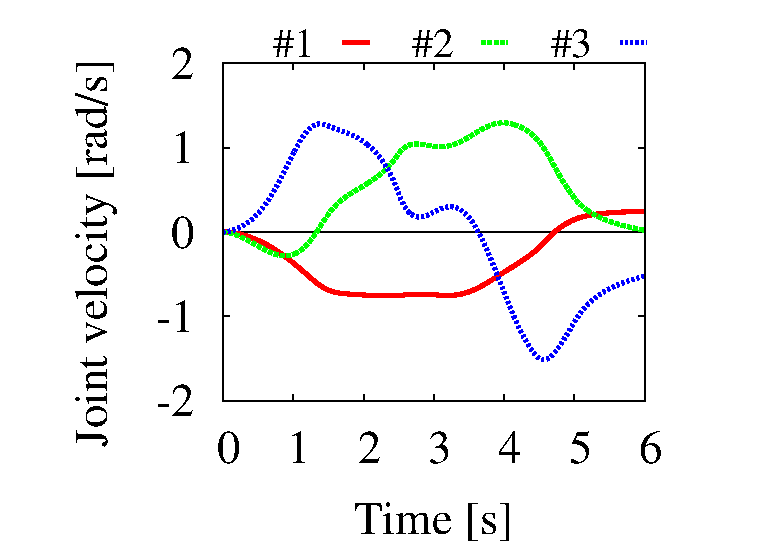
\includegraphics[width=1.0\linewidth]{fig/chapter7/mass/planar/10.eps}
  \end{minipage}
  \begin{minipage}{0.327\linewidth}
    \centering
    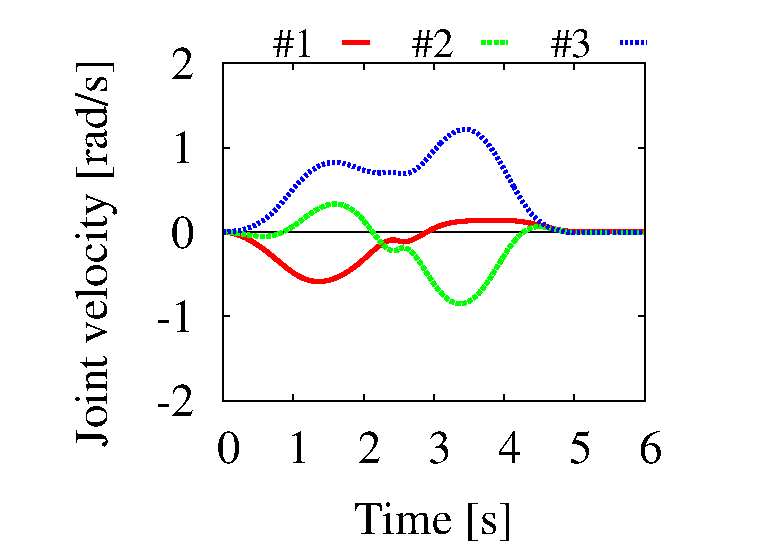
\includegraphics[width=1.0\linewidth]{fig/chapter7/mass/planar/100.eps}
  \end{minipage}
  \begin{minipage}{0.327\linewidth}
    \centering
    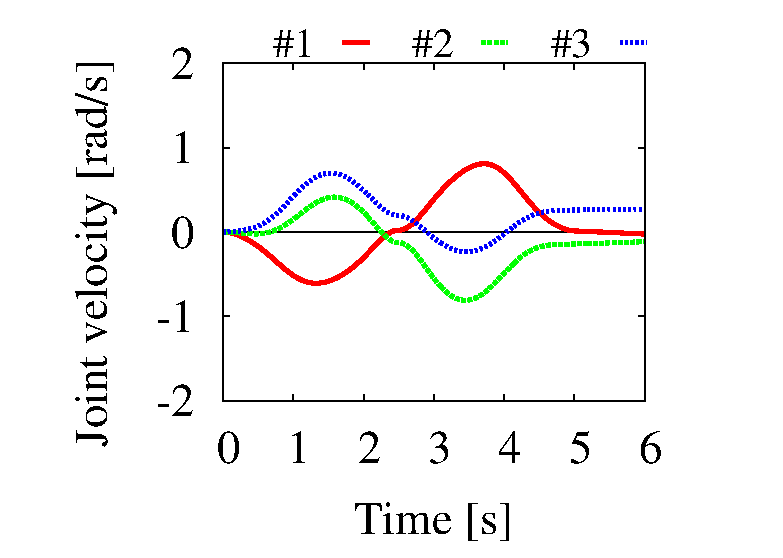
\includegraphics[width=1.0\linewidth]{fig/chapter7/mass/planar/1000.eps}
  \end{minipage}\\
  \vspace{1em}
  \begin{minipage}{0.327\linewidth}
    \centering
    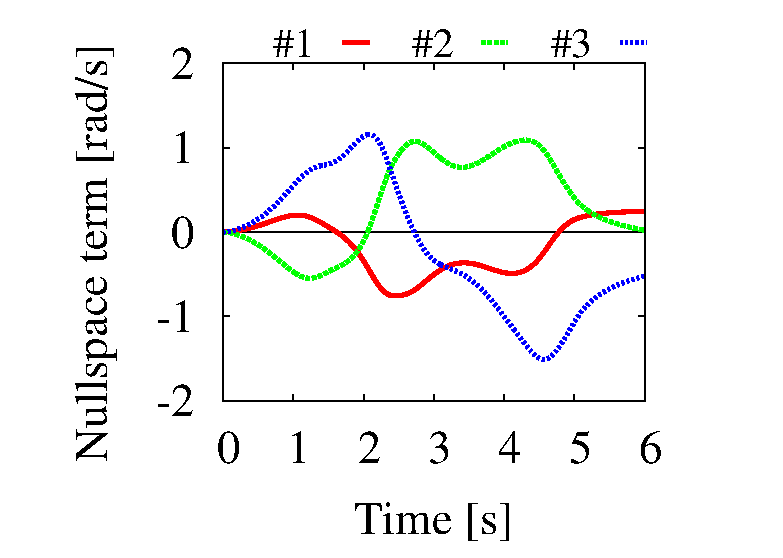
\includegraphics[width=1.0\linewidth]{fig/chapter7/mass/planar/10_null.eps}
    \footnotesize\par{\vspace{2mm}$10\unit{kg}$}
  \end{minipage}
  \begin{minipage}{0.327\linewidth}
    \centering
    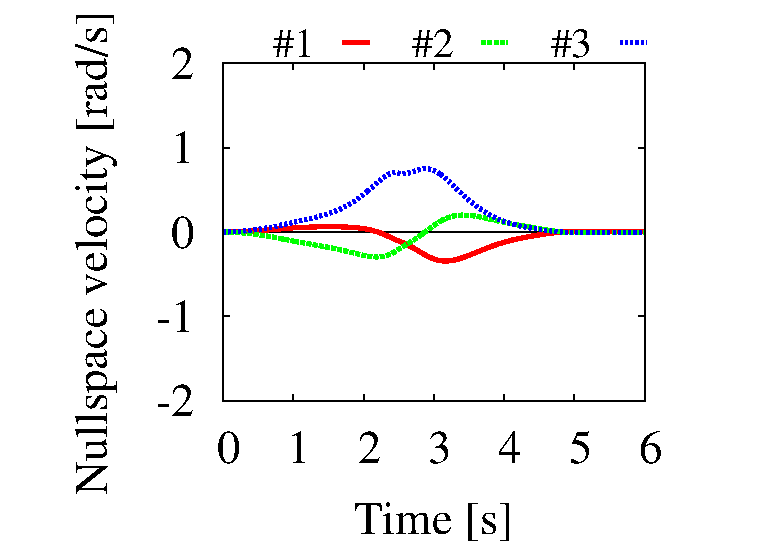
\includegraphics[width=1.0\linewidth]{fig/chapter7/mass/planar/100_null.eps}
    \footnotesize\par{\vspace{2mm}$100\unit{kg}$}
  \end{minipage}
  \begin{minipage}{0.327\linewidth}
    \centering
    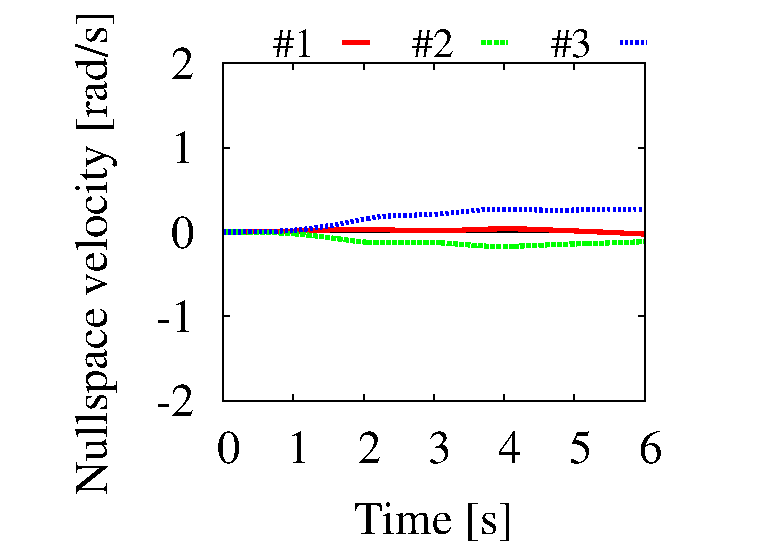
\includegraphics[width=1.0\linewidth]{fig/chapter7/mass/planar/1000_null.eps}
    \footnotesize\par{\vspace{2mm}$1000\unit{kg}$}
  \end{minipage}
  \caption{The time profiles of the joint velocity and the null-space velocity:
  the upper part represents the joint velocity; the lower part is the null-space velocity, respectively.}
  \label{fig:RES_3R_MOTION}
\end{figure}
% ---------------------------------------------------------------------
%
We show the time profile of the joint velocity and the null-space velocities in \fig{RES_3R_MOTION}.
In the figure,
the upper part shows the joint velocity with each constrained link mass;
the lower part is the null-space velocity, respectively.
From the results,
we can confirm that the null-space velocity is gradually decreasing,
when increasing the constrained link mass.
Our concern is the existence of the limit to which the motion under the RNS-based control converges,
when the constrained link mass/inertia moment become very large.
Actually, this limit exists and coincides with the minimum acceleration norm solution,
which is obtained from resolved acceleration control \cite{Luh1980} with the particular solution only.
In what follows,
we discuss this interesting feature.

%%%%%%%%%%%%%%%%%%%%%%%%
\subsection{Discussion}
%%%%%%%%%%%%%%%%%%%%%%%%

%%%%%%%%%%%%%%%%%%%%%%%%%%%%%%%%%%%%%%%%%%%%%%%%%
\subsubsection{Minimum acceleration constraint}
%%%%%%%%%%%%%%%%%%%%%%%%%%%%%%%%%%%%%%%%%%%%%%%%%
First, we obtain the condition of the minimum acceleration norm solution.
The equation describing the relation between end-effector acceleration
and joint acceleration is expressed in the following form:
%
% ---------------------------------------------------------------------
\begin{align}
  \dot{\mathcal{V}}_{e} = \bm{J}_{e}\thdd + \dot{\bm{J}}_{e}\thd
  \label{eq:ACC_EQ}
\end{align}
% ---------------------------------------------------------------------
%
% This equation must be satisfied under any conditions.
From the above equation,
given an end-effector acceleration,
the joint space can be divided into the two orthogonal subspaces as follows:
%
% ---------------------------------------------------------------------
\begin{align}
  \thdd = \bm{J}_{e}^{+}(\dot{\mathcal{V}}_{e} - \dot{\bm{J}}_{e}\thd) + \bm{P}_{J}\thdd_{a}
  \label{eq:MINIMUM_ACC}
\end{align}
% ---------------------------------------------------------------------
%
where $\bm{P}_{J} = \bm{E} - \bm{J}_{e}^{+}\bm{J}_{e}\R{n\times n}$ is the projection
onto the null-space of the Jacobian,
$\thdd_{a}\R{n}$ is an arbitrary vector with dimensions of joint acceleration.
The first term is the joint motion whose character is the minimum acceleration norm,
the second term is the orthogonal term.
We define the joint acceleration set $\mathcal{Q}_{J}$ as \eq{MINIMUM_ACC}.
The motion decomposition in \eq{MINIMUM_ACC}
is referred to as the resolved acceleration control.

%%%%%%%%%%%%%%%%%%%%%%%%%%%%%%%%%%%
\subsubsection{The RNS constraint}
%%%%%%%%%%%%%%%%%%%%%%%%%%%%%%%%%%%
Let us recall the constraint under RNS-based control as follows:
%
% ---------------------------------------------------------------------
\begin{align}
  \hthdd = -\hbm{M}_{Al}^{+}(\hbm{M}_{A}\dot{\hmathc{V}}_{A} + \hmathc{C}_{A}) +
  \hbm{M}_{Al}^{+}\hbm{T}\mathcal{F}_{B} + \hbm{P}_{RNS}\hthdd_{a}\label{eq:RNS_CONST_ACC}
\end{align}
% ---------------------------------------------------------------------
%
Note that we assume zero gravity environments without losing generality.
Among these acceleration terms,
we define a joint acceleration set related to the RNS-constraint as follows:
%
% ---------------------------------------------------------------------
\begin{align}
  \mathcal{Q}_{M_{Al}} = \{\hthdd\R{n}| 
  \hthdd = -\hbm{M}_{Al}^{+}(\hbm{M}_{A}\dot{\hmathc{V}}_{A} + \hmathc{C}_{A}) + \hbm{P}_{RNS}\hthdd_{a}\}
\end{align}
% ---------------------------------------------------------------------
%
This set consists of the accelerations appearing in \eq{RNS_CONST_ACC} except
the acceleration related to the constrained force.
Namely, $\mathcal{Q}_{M_{Al}}$ represents the acceleration set that is satisfied with
a completely free-floating model.

%%%%%%%%%%%%%%%%%%%%%%%%%%%%%%%%%
\subsubsection{The interpretation}
%%%%%%%%%%%%%%%%%%%%%%%%%%%%%%%%%
First, we assume that the order of the constrained link mass is the same as that of the other links mass.
In this case, $\mathcal{Q}_{M_{Al}}$ must differ from $\mathcal{Q}_{J}$, generally.
Then, the constrained force related term acts to make the acceleration obtained from the RNS
belong to $\mathcal{Q}_{J}$.
The geometrical interpretation is shown in \fig{GEO}~(a).
%
% ---------------------------------------------------------------------
\begin{figure}[t]
  \centering
  \begin{minipage}{1.0\linewidth}
    \centering
    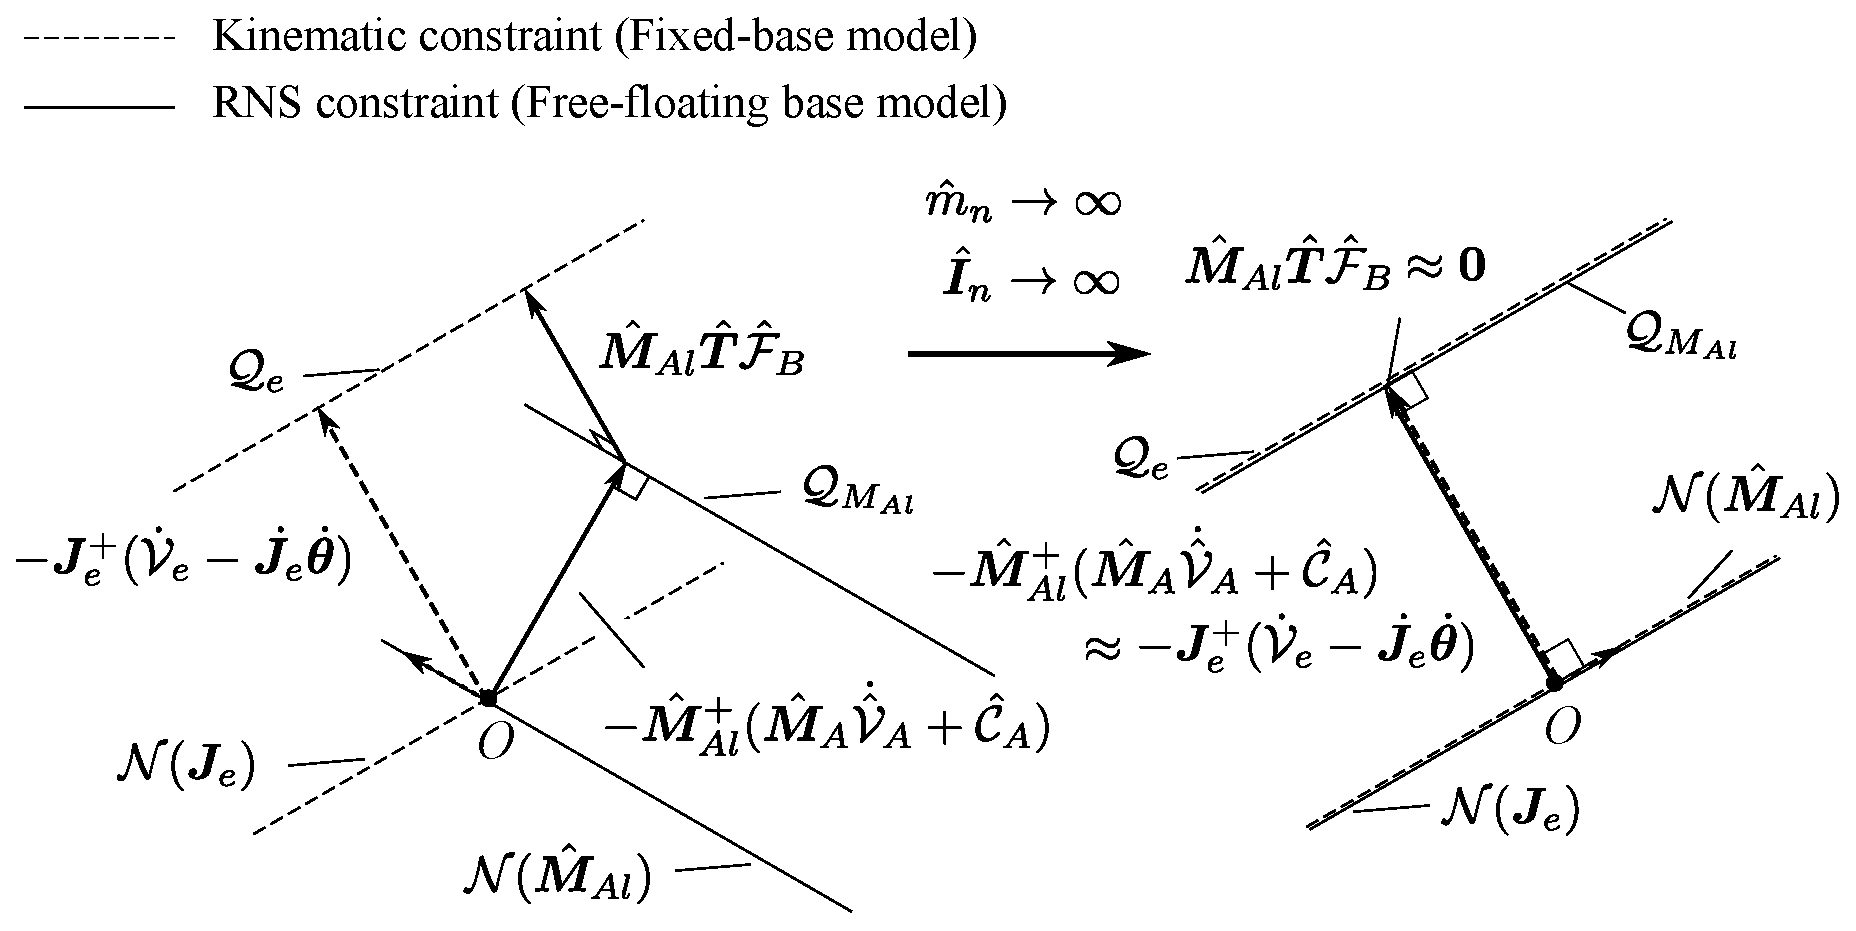
\includegraphics[width=1.0\linewidth]{fig/chapter7/mass/geo.eps}
    \vspace{0mm}
    \footnotesize\par{(a) \hspace{20em} (b)}
  \end{minipage}
  \caption{A geometrical interpretation of the RNS constraint:
  (a) with a small mass of the constrained link and (b) with a large value of the mass.}
  \label{fig:GEO}
\end{figure}
% ---------------------------------------------------------------------
%
Next, we consider the case when the constrained link mass and the inertia moment takes a huge value.
In this case, the linear and angular velocity of the constrained link become zero,
according to the momenta conservation laws, as follows:
%
% ---------------------------------------------------------------------
\begin{align}
  \hat{\bm{v}}_{n} &= \lim_{\hat{m}_{n} \rightarrow \infty}\frac{1}{\hat{m}_{n}}\sum_{i=0}^{n-1}\hat{m}_{i}\hat{\bm{v}}_{i}
  = \bm{0}\\
  \hat{\bm{\omega}}_{n} &= \lim_{\hat{\bm{I}}_{n} \rightarrow \infty}
  \frac{1}{\hbm{I}_{n}}\sum_{i=0}^{n-1}\{\hat{\bm{I}}_{i}\hat{\bm{\omega}}_{i} + \hat{m}_{i}\hat{\bm{r}}_{i}^{\times}\hat{\bm{v}}_{i}\} 
  = \bm{0}
\end{align}
% ---------------------------------------------------------------------
%
Therefore,
the free-floating base robot behaves as an $n$-link fixed
base robot even if there is no constrained force.
This means that $\mathcal{Q}_{M_{Al}}$ gradually converges to $\mathcal{Q}_{J}$,
when increasing the value of the constrained link mass.
The interpretation is shown in \fig{GEO}~(b).
Consequently,
the motion under RNS-based control coincides with that under resolved acceleration control,
i.e.\ minimum acceleration norm.

%%%%%%%%%%%%%%%%%%%%%%%%%
\subsection{Verification via numerical simulations}
%%%%%%%%%%%%%%%%%%%%%%%%%
In what follows,
we verify the character through numerical simulations with the planar model.
We compare a specific part of $\mathcal{Q}_{M_{Al}}$ with $\mathcal{Q}_{J}$
under $\hthdd_{a} = \bm{0}$ in the both set.
The simulation conditions are the same ones used in \sec{ANALYSIS_MOTION}.
To evaluate the equivalence,
we make use of the root mean square (RMS) of the motion error between
under the RNS-based control and the resolved acceleration control as follows:
%
% ---------------------------------------------------------------------
\begin{align}
  \mathrm{RMS}[\Delta \th] &= \sqrt{\frac{1}{t_{f} - t_{0}}\int_{t_{0}}^{t_{f}}\|\Delta \th(t)\|^{2}}\\
  \Delta \th(t) &= \th_{RNS}(t) - \th_{RA}(t)
  \label{eq:RMS}
\end{align}
% ---------------------------------------------------------------------
%
where $\th_{RNS}$ and $\th_{RA}$ stand for
the joint motion under the RNS-based control and the resolved acceleration control, respectively.
%
% ---------------------------------------------------------------------
\begin{figure}[t]
  \centering
  \begin{minipage}{0.75\linewidth}
    \centering
    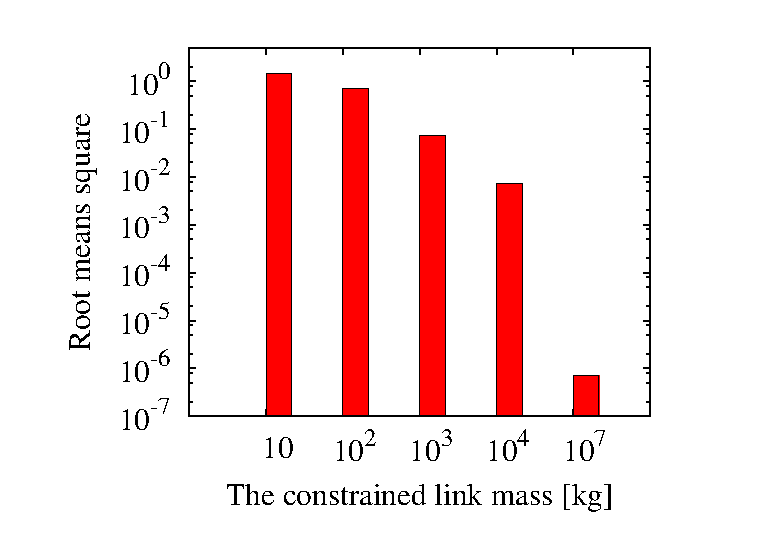
\includegraphics[width=1.0\linewidth]{fig/chapter7/mass/rms_planar.eps}
  \end{minipage}
  \caption{The root means square of the motion error.}
  \label{fig:RES_RMS}
\end{figure}
% ---------------------------------------------------------------------
%

The simulation results are displayed in \fig{RES_RMS}.
The simulations were conducted with some values of the constrained link mass.
In the graph,
note that $y$-axis is represented via log scale.
From the results,
we can confirm that the motion error described in \eq{RMS} is gradually reduced,
when increasing the value of the constrained link mass.
Hence, the character is proved.


%%%%%%%%%%%%%%%%%%%%%%%%%%%%%%%%%%%%%%%
\section{Stabilization of joint motion}
%%%%%%%%%%%%%%%%%%%%%%%%%%%%%%%%%%%%%%%
Despite acceleration-based kinematic control schemes have advantages in terms of
responsive and precise motion,
there is a problem with instability of the joint motion.
The problem has been discussed by several researchers \cite{ONeil2000,ONeil2002,Hollerbach1985}.
In particular, it has been pointed out that 
the local torque optimization frequently yields unstable behavior.
For this problem,
an important analysis that clarifies the mechanism of the instability was done in \cite{Maciejewski1991}.
In that work,
it was shown that the null-space acceleration/torque vectors that yield the local torque minimization
work as a positive feedback input on the null-space velocity.
As a result, instability can be observed.
To obtain a stable behavior of joint motion,
it is mentioned that global optimization is necessary for torque minimization \cite{Hollerbach1987}.
In the same work,
some redundancy resolution schemes were also compared with a three-link model.
These schemes are minimum acceleration norm, local torque minimization and
the weighted minimum acceleration norm with the inertia matrix.
Among them, the local torque minimization and the inertia weighted minimum acceleration schemes
became destabilized.
On the other hand,
the minimum acceleration norm did not become unstable, frequently.
However, the method also can be unstable under specific conditions.
An analysis indicated that all redundancy resolution schemes with dimension of acceleration
can become unstable \cite{Maciejewski1991}:
i.e.\ there is a finite escape time in all schemes.

As a different matter related to the instability,
it is well-known that the null-space velocities remain at the end of motion,
with acceleration based control methods.

To overcome these problems,
velocity based acceleration control methods have been focused on
by some researchers \cite{Ma1996,Watanabe2001,ShugenMa1996}.
The solution is obtained as the time differential of velocity based solutions.
The solution does not cause the instability
because of the property of the minimum velocity norm constraint.
In \cite{ShugenMa1996},
local torque minimization was carried out based on the velocity based methods.

As seen in \cha{FORMULATION} and \sec{ANALYSIS_MOTION},
residual joint velocity at the end of motion was observed.
% Under the RNS-based motion control,
% the same problem can happen as same as the kinematic schemes can.
To alleviate the problem,
we obtain the velocity based acceleration solution for the RNS-based control, in what follows.

%%%%%%%%%%%%%%%%%%%%%%%%%%%%%%%%%%%%%%%%%%%%%%%%%%%%%%%%
\subsection{Velocity-level based acceleration solution}
%%%%%%%%%%%%%%%%%%%%%%%%%%%%%%%%%%%%%%%%%%%%%%%%%%%%%%%%
We begin to formulate the solution, considering a velocity level equation.
In this case, the velocity level equation is the momentum equation.
The equation can be written as follows:
%
% ---------------------------------------------------------------------
\begin{align}
  \hbm{M}_{A}\dot{\hmathc{V}}_{A} + \hbm{M}_{Al}\hthd = \bm{0}
\end{align}
% ---------------------------------------------------------------------
%
We assume no interaction and zero gravity, for the sake of simplicity.
Given the assumption, we do not lose generality.
When considering zero null-space motion,
the joint velocity can be expressed as follows:
%
% ---------------------------------------------------------------------
\begin{align}
  \hthd = -\hbm{M}_{Al}^{+}\hbm{M}_{A}\hmathc{V}_{A}\label{eq:VEL_SOL}
\end{align}
% ---------------------------------------------------------------------
%
This equation implies the minimum velocity constraint.
Taking derivative of \eq{VEL_SOL} in terms of time,
we can obtain the velocity based acceleration solution as follows:
%
% ---------------------------------------------------------------------
\begin{align}
  \hthdd &= -\DT(\hbm{M}_{Al}^{+})\hbm{M}_{A}\hmathc{V}_{A} - \hbm{M}_{Al}^{+}(\dot{\hbm{M}}_{A}\hmathc{V}_{A}
  + \hbm{M}_{A}\dot{\hmathc{V}}_{A}) \notag \\
  &= -\hbm{M}_{Al}^{+}(\hbm{M}_{A}\dot{\hmathc{V}}_{A} + \hmathc{C}_{A})
  - \hbm{P}_{RNS}(\dot{\hbm{M}}_{Al}^{T}(\hbm{M}_{Al}\hbm{M}_{Al}^{T})^{-1}\hbm{M}_{A}\mathcal{V}_{A})
  \label{eq:VEL_ACC_SOL}
\end{align}
% ---------------------------------------------------------------------
%
where the time differential of the pseudoinverse can be obtained as follows \cite{Ma1996}:
%
% ---------------------------------------------------------------------
\begin{align}
  \DT(\hbm{M}_{Al}^{+}) &= -\hbm{M}_{Al}^{+}\dot{\hbm{M}}_{Al}\hbm{M}_{Al}^{+} +
  \hbm{P}_{RNS}\dot{\hbm{M}}_{Al}^{T}(\hbm{M}_{Al}\hbm{M}_{Al}^{T})^{-1}
\end{align}
% ---------------------------------------------------------------------
%

Comparing \eq{VEL_ACC_SOL} with \eq{RNS_CONST_ACC},
we can see that there is an additional acceleration term in \eq{VEL_ACC_SOL}, as follows:
%
% ---------------------------------------------------------------------
\begin{align}
  \hthdd = -\hbm{P}_{RNS}\dot{\hbm{M}}_{Al}^{T}(\hbm{M}_{Al}\hbm{M}_{Al}^{T})^{-1}\hbm{M}_{A}\mathcal{V}_{A}
\end{align}
% ---------------------------------------------------------------------
%
Equation \eq{VEL_ACC_SOL} is the minimum velocity solution in terms of acceleration.

%%%%%%%%%%%%%%%%%%%%%%%%%%%%%%%%%%%%%%%%%%%%%%%%%%%%%
\subsection{Verification via numerical simulations}
%%%%%%%%%%%%%%%%%%%%%%%%%%%%%%%%%%%%%%%%%%%%%%%%%%%%%
%
% ---------------------------------------------------------------------
\begin{figure}[t]
  \centering
  \begin{minipage}{0.7\linewidth}
    \centering
    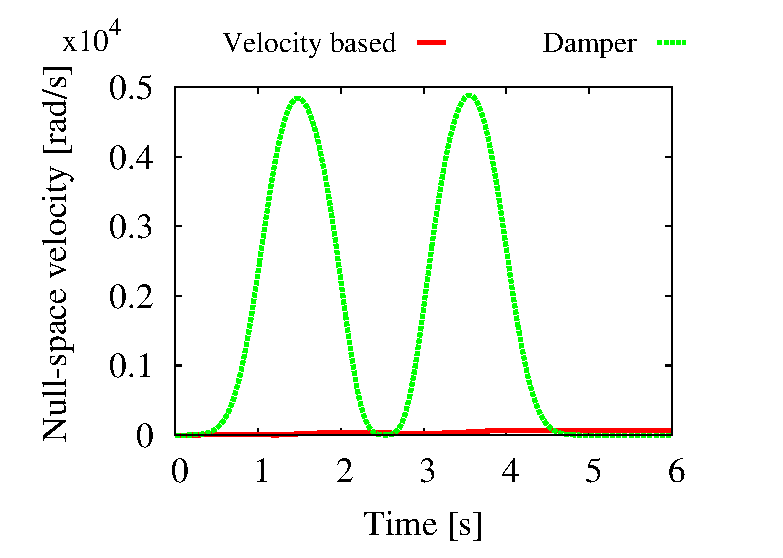
\includegraphics[width=1.0\linewidth]{fig/chapter7/stabilize/nullspace.eps}
  \end{minipage}
  \caption{Time profile of the Euclidean norm of the null-space velocity:
  the line in red represents the velocity based acceleration solution;
the line in green stands for the velocity with the damper.}
  \label{fig:RES_VEL}
\end{figure}
% ---------------------------------------------------------------------
%
Here, we verify the validness of the obtained solution through numerical simulations with
the three-link planar model.
The simulation conditions and the desired motion of the end-effector were
the same ones that are used in \sec{ANALYSIS_MOTION}.
The constrained link mass was set to $10^{4}\unit{kg}$.

To evaluate the validness,
the resultant joint velocity is decomposed into the two parts as follows:
%
% ---------------------------------------------------------------------
\begin{align}
  \thd = (\bm{E} - \hbm{P}_{RNS})\thd + \hbm{P}_{RNS}\thd\label{eq:DECOMPOSED}
\end{align}
% ---------------------------------------------------------------------
%
Under the minimum velocity norm condition,
the second term in \eq{DECOMPOSED} must be zero.
Hence, we make use of the Euclidean norm of the second term as the cost function.
To obtain a comparative evaluation,
we executed a simulation with adding a damping term into the null-space acceleration in \eq{RNS_CONST_ACC}:
$\hthdd_{a} = -\bm{K}_{d}\hthd$.
The value of the damper $\bm{K}_{d} = \mathrm{diag}(k_{d},k_{d},k_{d})$ was a high limit without
causing instability: $k_{d} = 2770 \unit{s^{-1}}$.


We show the time profiles of the Euclidean norms in \fig{RES_VEL}.
In the graph,
the line in red represents the velocity-level based solution;
the line in green stands for the result with the damping term.
Comparing with these results,
we can see that the order of the null-space velocity with the damping is much larger than
that with the velocity level-based solution.
Hence, we can conclude that the proposed stabilization term has a good potential
in terms of joint stabilization.


% %%%%%%%%%%%%%%%%%%%%%%%%%%%%%%%%%%%%%%%
% \section{Joint motion comparison}
% %%%%%%%%%%%%%%%%%%%%%%%%%%%%%%%%%%%%%%%
% On redundant manipulators,
% while the task-space behaviors are identical,
% the joint-space behaviors, on the other hand, seem to be quite different,
% as seen in \cha{FORMULATION}.
% % Especially a large joint velocity was observed the OS formulation based control.
% % This results would be related to the inertia-weighted generalized inverse of the Jacobian.
% % This section focuses on joint motions under the OS formulation based control.
% This section compares three redundancy resolution schemes:
% (i) resolved acceleration control with minimum acceleration norm (RA-C)
% (ii) resolved acceleration control with inertia-weighted minimum acceleration norm (RAIW-C) and
% (ii) the OS formulation based control (OS-C).
% The joint motion under RA-C is identical to that under the RNS based controller when the constrained link mass/inertia moment
% are massive as described above.

% Joint accelerations under each schemes are represented as follows:
% %
% % ---------------------------------------------------------------------
% \begin{align}
%   \thdd_{RA}& = \bm{J}_{e}^{+}(\dot{\mathcal{V}}_{e}^{ref} - \dot{\bm{J}}_{e}\thd)\\
%   \thdd_{RAIW} &= \bm{J}_{e}^{M+}(\dot{\mathcal{V}}_{e}^{ref} - \dot{\bm{J}}_{e}\thd)\\
%   \thdd_{OS} &= \bm{J}_{e}^{M+}(\dot{\mathcal{V}}_{e}^{ref} - \dot{\bm{J}}_{e}\thd) +
%   (\bm{E} - \bm{J}_{e}^{M+}\bm{J}_{e})\bm{M}_{l}^{-1}(\bm{c}_{l} + \bm{g}_{l})
% \end{align}
% % ---------------------------------------------------------------------
% %
% where $\thdd_{RA}$, $\thdd_{RAIW}$ and $\thdd_{OS}$ stand for
% the joint accelerations under RA-C, RAIW-C and OS-C, respectively.
% $\thdd_{OS}$ is obtained from \eq{TAU_OS1} and \eq{EOM_JOINT}.
% We should note that gravity force induces a null-space motion under OS-C.
% Therefore, even the end-effector is motionless,
% a cyclic null-space motion happens as shown in \fig{OS_CYCLIC}.
% %
% % ---------------------------------------------------------------------
% \begin{figure}[t]
%   \centering
%   \begin{minipage}{0.45\linewidth}
%     \centering
%     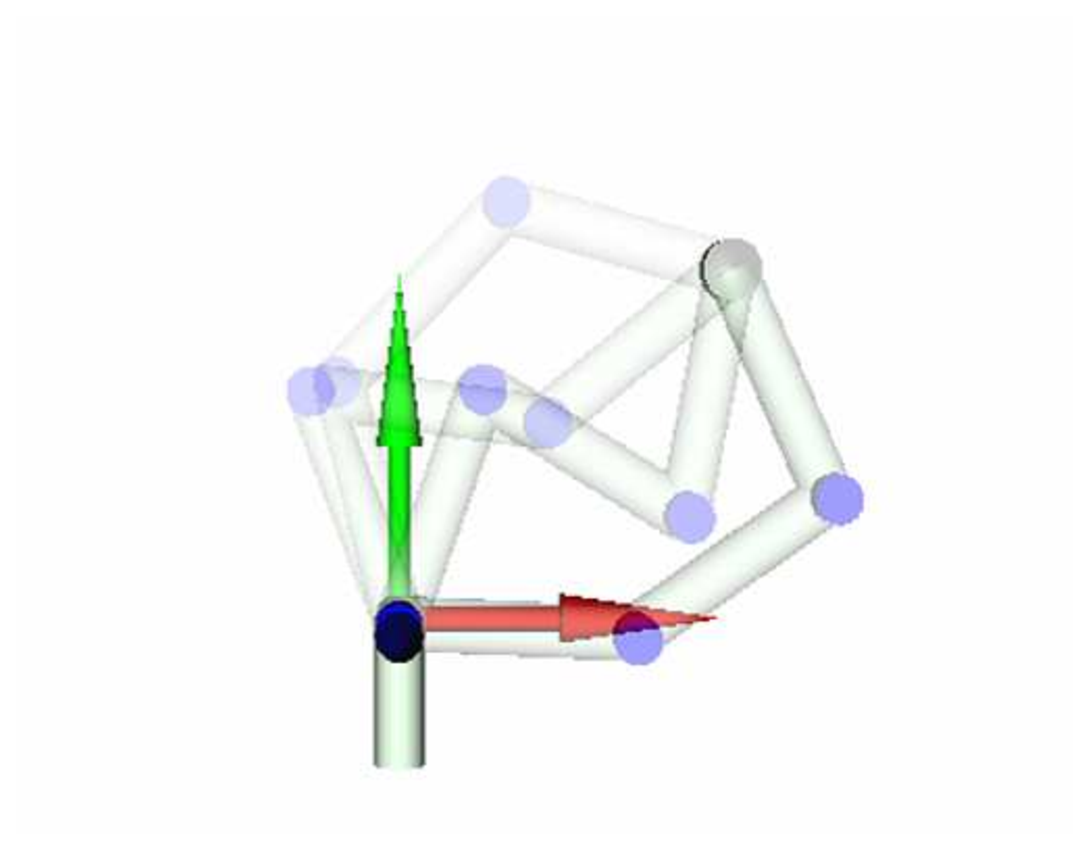
\includegraphics[width=1.0\linewidth]{fig/chapter7/comparison/OSF/gravity_figure.eps}
%   \end{minipage}
%   \begin{minipage}{0.45\linewidth}
%     \centering
%     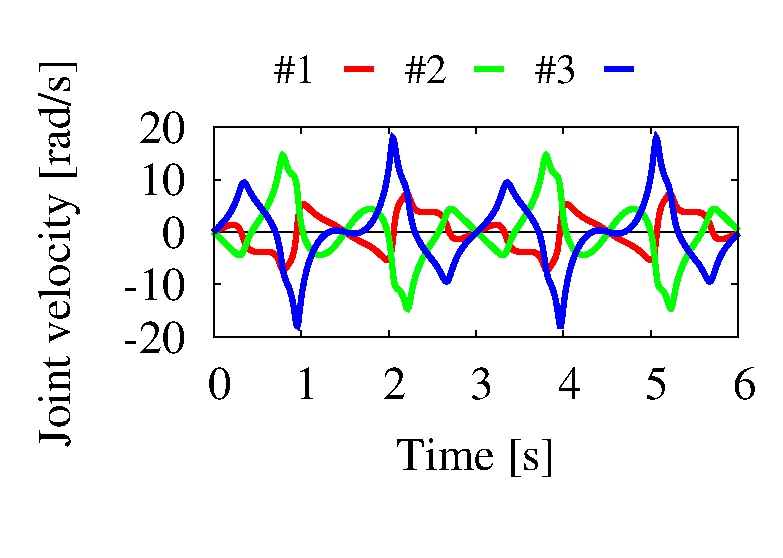
\includegraphics[width=1.0\linewidth]{fig/chapter7/comparison/OSF/gravity_graph.eps}
%   \end{minipage}
%   \caption{Cyclic motion induced by gravity compensation under the OS formulation.}
%   \label{fig:OS_CYCLIC}
% \end{figure}
% % ---------------------------------------------------------------------
% %
% To avoid this undesirable behavior,
% the gravity compensation should be executed by a different way.
% Hereafter, we assume zero gravity for the sake of simplicity.



%%%%%%%%%%%%%%%%%%%%
\section{Summary}
%%%%%%%%%%%%%%%%%%%%
In this chapter,
we discussed the joint motion under RNS-based control.
As an interesting character,
we found out that the joint motion under RNS-based control converges to
that under resolved acceleration control, increasing the constrained link mass.

As a different issue,
we dealt with the instability of the joint motion
arising from non-integrability of acceleration-level based control methods.
We derived a velocity-level based acceleration solution to obtain a stable motion.
This solution was verified via numerical simulation;
that has a potential in terms of joint stabilization.








%**********************************************************************
%
%
%%% Local Variables:
%%% mode: latex
%%% TeX-master: "./main"
%%% End: